\documentclass{beamer}

\mode<presentation>
{
  \usetheme{Darmstadt}
  \setbeamercovered{dynamic}
}


\usepackage[english]{babel}
\usepackage[latin1]{inputenc}

\usepackage{times}
\usepackage[T1]{fontenc}
\usepackage{tikz}
\usepackage{amsmath}
\usepackage{verbatim}
\usepackage{subfigure}
\usepackage{graphicx}
\usepackage{wrapfig}
\usetikzlibrary{arrows,shapes}
\tikzstyle{decision} = [diamond, draw, text width=4.5em, text badly centered, node distance=3cm, inner sep=0pt]
\tikzstyle{block} = [rectangle, draw, text width=20em, text centered, rounded corners, minimum height=4em]
\tikzstyle{smallblock} = [rectangle, draw, text width=8em, text centered, rounded corners, minimum height=4em]
\tikzstyle{longblock} = [rectangle, draw, text width=6em, text centered, rounded corners, minimum height=8em]
\tikzstyle{elongatedblock} = [rectangle, draw, text width=7em, text centered, rounded corners, minimum height=2em]
% Or whatever. Note that the encoding and the font should match. If T1
% does not look nice, try deleting the line with the fontenc.


\title[Title] % (optional, use only with long paper titles)
{Uncertainty Propagation in Nonlinear Dynamic Systems using Adaptive Gaussian Sum Filter}

%\subtitle
%{Include Only If Paper Has a Subtitle}

\author
{Kumar ~Vishwajeet}

\institute
{
  Department of Mechanical \& Aerospace Engineering\\
  University at Buffalo
}

\date[CFP 2011] % (optional, should be abbreviation of conference name)
{Project Proposal for Optimal Estimation, Spring 2011}

\subject{Optimal Estimation}

% If you have a file called "university-logo-filename.xxx", where xxx
% is a graphic format that can be processed by latex or pdflatex,
% resp., then you can add a logo as follows:

% \pgfdeclareimage[height=0.5cm]{university-logo}{university-logo-filename}
% \logo{\pgfuseimage{university-logo}}



% Delete this, if you do not want the table of contents to pop up at
% the beginning of each subsection:
%\AtBeginSubsection[]
%{
  %\begin{frame}<beamer>{Outline}
    %\tableofcontents[currentsection,currentsubsection]
  %\end{frame}
%}


% If you wish to uncover everything in a step-wise fashion, uncomment
% the following command:

\beamerdefaultoverlayspecification{<+->}


\begin{document}
\tikzstyle{every picture}+=[remember picture]

\begin{frame}
  \titlepage
\end{frame}

%\begin{frame}{Outline}
  %\tableofcontents
   %You might wish to add the option [pausesections]
%\end{frame}


% Structuring a talk is a difficult task and the following structure
% may not be suitable. Here are some rules that apply for this
% solution:

% - Exactly two or three sections (other than the summary).
% - At *most* three subsections per section.
% - Talk about 30s to 2min per frame. So there should be between about
%   15 and 30 frames, all told.

% - A conference audience is likely to know very little of what you
%   are going to talk about. So *simplify*!
% - In a 20min talk, getting the main ideas across is hard
%   enough. Leave out details, even if it means being less precise than
%   you think necessary.
% - If you omit details that are vital to the proof/implementation,
%   just say so once. Everybody will be happy with that.

\section{Motivation}

%\subsection{The Basic Problem That We Studied}

\begin{frame}{Nonlinear Filtering}{Methods in use}
  % - A title should summarize the slide in an understandable fashion
  %   for anyone how does not follow everything on the slide itself.
\tikzstyle{na} = [baseline=-.5ex]
\begin{enumerate}
  \item
    Kalman Filter - Originally for Gaussian Linear Systems
  \begin{itemize}
    \item
    \fontsize{8}{10}\selectfont Eliminate Gaussian Assumption: \fontsize{6}{10}\selectfont Approximate a non-Gaussian pdf with weighted sum of n number of Gaussian pdf \\
    \begin{equation}
    \begin{split}
    \fontsize{6}{10}\selectfont
    \hat{p}(t,x(t))      & = \sum_{i=1}^{n}w_i \mathcal{N} (x(t)| \mu_i(t),P_i(t))\\
    \sum_{i=1}^{n} w_i(t)& = 1;   w_i(t) \geq 0, \forall i
    \end{split}
    \end{equation}
  \end{itemize}
  \item
    Nonlinear Systems
    \pause
    \tikz[na] \node[coordinate] (n1) {};
    \begin{figure}[h]
 \begin{center}
  \fontsize{6}{10}\selectfont
 \subfigure[\fontsize{8}{10}\selectfont Extended Kalman Filter(EKF)]{
  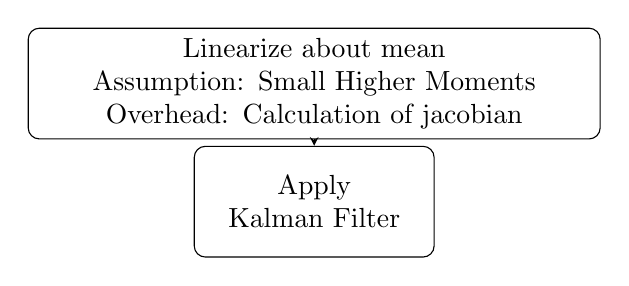
\begin{tikzpicture}[node distance=1.5cm, auto, >=stealth]
   \node[block] (a)                                     {Linearize about mean \\ Assumption: Small Higher Moments \\ Overhead: Calculation of jacobian};
   \node[smallblock] (b)  [below of=a]                       {Apply Kalman Filter};
   \draw[->] (a) -- (b);
  \end{tikzpicture}
  \label{flowchart}}
  \fontsize{6}{10}\selectfont
  \subfigure[\fontsize{8}{10}\selectfont Unscented Kalman Filter(UKF)]{
  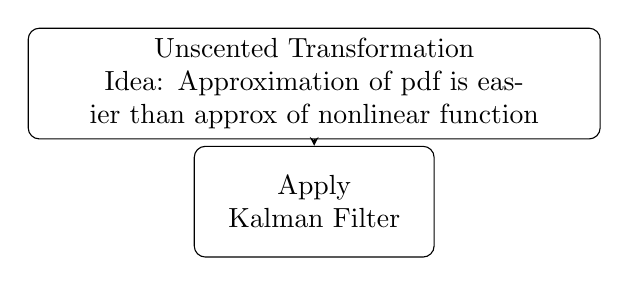
\begin{tikzpicture}[node distance=1.5cm, auto, >=stealth]
    \node[block] (a)                                     {Unscented Transformation \\ Idea: Approximation of pdf is easier than approx of nonlinear function};
   \node[smallblock] (b)  [below of=a]                       {Apply Kalman Filter};
   \draw[->] (a) -- (b);
  \end{tikzpicture}
  \label{flowchart}}
 \end{center}
 \end{figure}
 \end{enumerate}
\end{frame}

\begin{frame}{Nonlinear Filtering}{Algorithm/Flowchart}
\begin{block}{Algorithm}
     \fontsize{6}{10}\selectfont
      for t = $t_0$ to $t_{end}$ \\
      {\hspace{3pt}
            Propagate mean and covariance of each Gaussian component using EKF/UKF.\\
      \hspace{3pt}
            If measurement is available \\
            \hspace{6pt}
                    do measurement update \\
            \hspace{6pt}
                    do Weight update \\
      end}
\end{block}
\begin{block}{Flowchart}
\begin{figure}
\fontsize{6}{10}\selectfont
 \begin{center}
  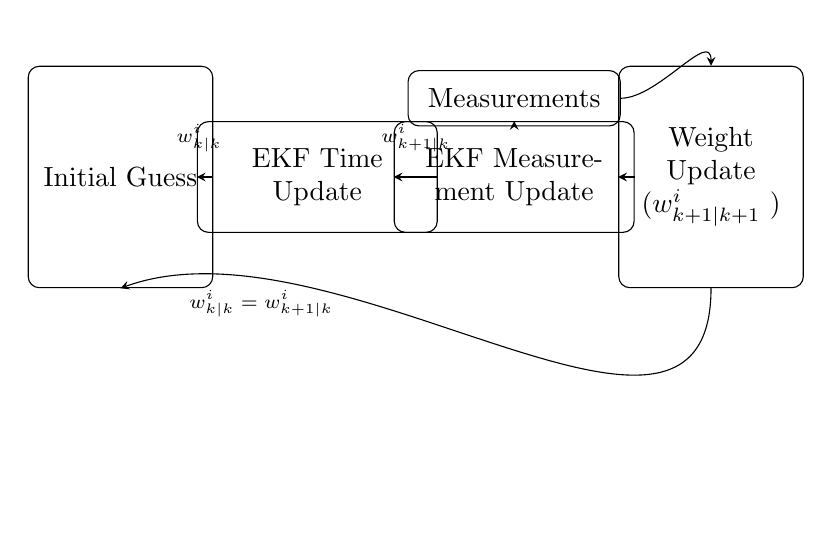
\begin{tikzpicture}[node distance=2.5cm, auto, >=stealth]
   % nodes
   \node[longblock] (a)                                     {Initial Guess};
   \node[smallblock] (b)  [right of=a]                       {EKF Time Update};
   \node[smallblock] (c)  [right of=b]                       {EKF Measurement Update};
   \node[longblock] (d)  [right of=c]                       {Weight Update\\($w_{k+1|k+1}^i$ )};
   \node[elongatedblock] (e)  [above of=c, node distance=1cm] {Measurements};

   % edges
   \draw[->] (a) -- (b) node [xshift=-1.5cm,yshift=0.20cm,above] {\fontsize{7}{10}\selectfont {$w_{k|k}^i$}};
   \draw[->] (b) -- (c) node [xshift=-1.25cm,yshift=0.20cm,above] {\fontsize{7}{10}\selectfont {$w_{k+1|k}^i$}};
   \draw[->] (c) -- (d);
   \draw[->] (e) -- (c);
   \draw[->] (d.south) to [out=270,in=20] (a.south)node [yshift=-0.2cm,xshift=0.75cm,right] {\fontsize{7}{10}\selectfont {$w_{k|k}^i = w_{k+1|k}^i$}};
   \draw[->] (e.east) to [out = 0,in = 90] (d.north);
   \end{tikzpicture}
   \label{flowchart}
 \end{center}
\end{figure}
 \end{block}
\end{frame}


\begin{frame}{Adaptive gaussian Sum Filter(AGSF)}
\begin{itemize}
    \item
    Measurements are not available frequently
    \item
    Large Uncertainty
   \item
   Forecast weight Update:\fontsize{7}{10}\selectfont Minimize the error between the pdf using Gaussian sum approximation and the true pdf generated by solving Chapman Kolmogorov equation (CKE). The problem reduces to a convex quadratic optimization which guarantees convergence.
\end{itemize}
\begin{block}{Flowchart}
\begin{figure}
\fontsize{6}{10}\selectfont
 \begin{center}
  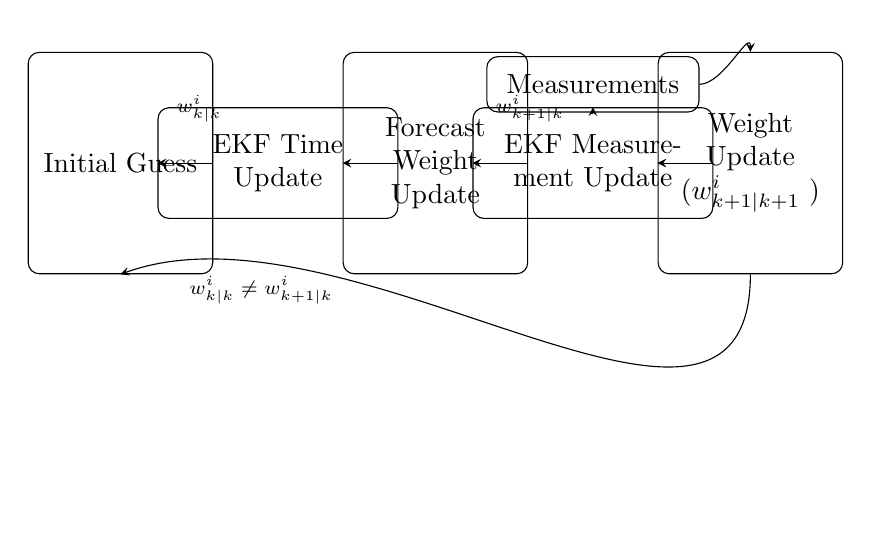
\begin{tikzpicture}[node distance=2cm, auto, >=stealth]
   % nodes
   \node[longblock] (a)                                     {Initial Guess};
   \node[smallblock] (b)  [right of=a]                       {EKF Time Update};
   \node[longblock] (c)  [right of=b]                       {Forecast Weight Update};
   \node[smallblock] (d)  [right of=c]                       {EKF Measurement Update};
   \node[longblock] (e)  [right of=d]                       {Weight Update\\($w_{k+1|k+1}^i$ )};
   \node[elongatedblock] (f)  [above of=d, node distance=1cm] {Measurements};

   % edges
   \draw[->] (a) -- (b) node [xshift=-1cm,yshift=0.40cm,above] {\fontsize{7}{10}\selectfont {$w_{k|k}^i$}};
   \draw[->] (b) -- (c);
   \draw[->] (c) -- (d) node [xshift=-0.80cm,yshift=0.40cm,above] {\fontsize{7}{10}\selectfont {$w_{k+1|k}^i$}};
   \draw[->] (d) -- (e);
   \draw[->] (f) -- (d);
   \draw[->] (e.south) to [out=270,in=20] (a.south) node [yshift=-0.2cm,xshift=0.75cm,right] {\fontsize{7}{10}\selectfont {$w_{k|k}^i \not= w_{k+1|k}^i$}};
   \draw[->] (f.east) to [out = 0,in = 90] (e.north);
   \end{tikzpicture}
   \label{flowchart}
 \end{center}
\end{figure}
 \end{block}
\end{frame}

\section{Two Body Problem}

\subsection{Equations of motion}

\begin{frame}
\begin{block}{Equation of motion}
\textbf{r = $R_2$ - $R_1$}\\
$m_1\ddot{R_1}=\frac{Gm_1m_2}{r^3}\textbf{r} + f_1$
\hspace{20 mm}
$m_1\ddot{R_2}=\frac{-Gm_1m_2}{r^3}\textbf{r} + f_2$ \\
$\ddot{R_1}=\frac{Gm_2}{r^3}\textbf{r} + \frac{f_1}{m_1}$
\hspace{30 mm}
$\ddot{R_2}=\frac{-Gm_1}{r^3}\textbf{r} + \frac{f_2}{m_2}$ \\
$\ddot{R_2}-\ddot{R_1}=\frac{G(m_1+m_2)}{r^3}\textbf{r} + a_d$ \\
$\ddot{\textbf{r}}=\frac{-\mu}{r^3}\textbf{r} + a_d$ \\
 \end{block}
 \begin{center}  
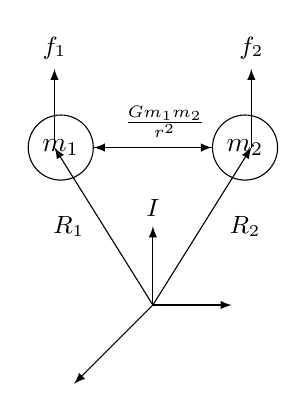
\begin{tikzpicture}
\draw (1,2) node[anchor=east,circle,
draw] (A) {$m_1$} -- (2.5,2) node[anchor=west,
circle,draw] (B) {$m_2$};
\draw[-latex] (A.east) -- (B.west);
\draw[-latex] (B.west) -- (A.east) node [xshift=0.9cm,above] {\small $\frac{Gm_1m_2}{r^2}$}; ;
\draw[-latex] (0.5,2) -- (0.5,3) node [above] {\small $f_1$};
\draw[-latex] (3,2) -- (3,3) node [above] {\small $f_2$};
\draw[-latex] (1.75,0.0) -- (0.5,2) node [yshift=-1cm,xshift=0.5cm,left] {\small $R_1$};
\draw[-latex] (1.75,0.0) -- (3,2) node [yshift=-1cm,xshift=-0.4cm,right] {\small $R_2$};
\draw[-latex] (1.75,0.0) -- (1.75,1) node [above] {\small $I$};
\draw[-latex] (1.75,0.0) -- (0.75,-1);
\draw[-latex] (1.75,0.0) -- (2.75,0.0);
\makebox[6cm]{text}
\end{tikzpicture}
\end{center}
\end{frame}


\section*{Problem Statement}

\begin{frame}{Problem Statement}
\begin{enumerate}
  \item
    Large Uncertainty exist in the initial states.
  \begin{itemize}
    \item
    Use UKF for propagation of mean and covariance.
    \item
    Use 6n+1 Gaussian components for approximation.
    \item
    Use parallel computing to get quick results.
  \end{itemize}
  \item
    Use Monte carlo simulations to validate the results.
  \end{enumerate}
\end{frame}



% All of the following is optional and typically not needed.
\appendix
\section<presentation>*{\appendixname}
\subsection<presentation>*{References}

\begin{frame}[allowframebreaks]
  \frametitle<presentation>{References}

  \begin{thebibliography}{10}

  \beamertemplatebookbibitems
  % Start with overview books.

  \bibitem{Author1990}
    G.~Terejanu,P.~Singla, T.~Singh, P. Scott
    \newblock {\em Adaptive Gaussian Filter for Nonlinear Bayesian Estimation}.
    \newblock IEEE Transactions on Automatic Control


  \beamertemplatearticlebibitems
  % Followed by interesting articles. Keep the list short.

  \bibitem{Someone2000}
    H.~Schaub, J.~Junkins.
    \newblock On this and that.
    \newblock {\em Analytical Mechanics of Space systems},
    \newblock AIAA Education Series

  \end{thebibliography}
\end{frame}

\end{document}


